Now we will see an interesting application of scientific visualization which can also be an excellent test case for approaches in Chapter~\ref{Chapter21}: creation of three-dimensional models from \textit{medical images}.
In fact, this is a good application, because the typical medical image contains a large amount of data. As pointed out by \cite{Stytz}, the average CT procedure generates more than 2 million voxels (see Section~\ref{sec13:medicalImaging}) per patient examination and also other imaging techniques produce similar amounts of data. Moreover algorithms used for 3D medical imaging have great computational cost, even at moderate resolution.\\
\newline
A lot of the material that will be presented in this Chapter comes from \cite{Birkfellner}, which represents an excellent source for the image processing world applied to medicine. It describes also the importance of the use of radiological images for clinical research. In fact, the author points out that their applications range from neuroscience, biomechanics and biomedical engineering to clinical routine tasks such as: the visualization of huge datasets provided by computed tomography systems, the manufacturing of patient-specific prostheses for orthopedic surgery or the planning of dose distributions in oncology. Here we will present the basis for understanding of techniques used to produce the images.

\section{Medical imaging basis}\label{sec13:medicalImaging}

\subsection{The electromagnetic spectrum}

Whoever wants to seriously study medical imaging should have a basic knowledge about the \textit{electromagnetic spectrum}. In fact, most images are generated by recording physical properties of tissues that are exposed by a certain type of electromagnetic (or sometimes mechanical) solicitation. Every radiation consists of \textit{photons} (little "particles of lights") with an energy equal to $E = h\nu$ where \textit{h} is the \textit{Planck constant} ($6.626 \cdot 10^{-34} Js$) and $\nu$ is the frequency of the wave. How we can see, as \textit{h} is a constant the energy of a wave is entirely described by its frequency. As a consequence, \cite{Birkfellner} uses the electromagnetic radiation frequencies for the definition of the following classification:
\begin{itemize}
 \item $1-10^{4}$ Hz: it is the range of frequency of alternating current and it is used for \textbf{electrical impedance tomography}
 \item $10^{4}-10^{8}$ Hz: frequencies used for broadcasting and for the \textbf{magnetic resonance imaging (MRI)}
 \item $10^{8}-10^{12}$ Hz: microwaves used in oven, they are not used in medical imaging
 \item $10^{12}-7 \cdot 10^{14}$ Hz: these are the frequencies of the infrared, used for \textbf{infrared imaging}
 \item $4.6 \cdot 10^{14}-6.6 \cdot 10^{14}$ Hz: spectrum of visible light. It is used for \textbf{light microscopy} and for \textbf{histological imaging}, \textbf{endoscopy} and \textbf{optical coherence tomography} 
 \item $4 \cdot 10^{14}-10^{18}$ Hz: ultraviolet frequencies which are used in \textbf{fluorescence imaging}
 \item $10^{18}-10^{18}$ Hz: X-rays, which are used for the \textbf{x-rays images}
 \item Beyond $10^{20}$ Hz: these are the frequencies of $\gamma-$radiation, which is usually a product of radioactive decay. Since $\gamma-$radiation may penetrate tissues easily it is widely used in nuclear medicine (\textbf{SPECT} and \textbf{PET}).
\end{itemize}

As we can see, medical imaging uses a large part of the electromagnetic spectrum. However there is a widespread imaging modality that relies on a different physical principle: \textbf{ultrasound}. These techniques will be studied further on.\\

\subsection{Image representation}

A digital image is represented by numerical values associated with positions in a regular grid. A single position is usually called \textbf{pixel} and its value is a gray value or a color. Anyhow, in medical image processing we often have three-dimensional representations. So, we can associate the numerical value mentioned above with a point in a three-dimensional space calling it \textbf{voxel}. Therefore an image is a discrete mathematical function which maps a vector from a two (or three) dimensional space to a number. As we can read in~\cite{Birkfellner}, formally speaking an image is represented as:
\begin{equation}
 I(x, y, z) = \rho
\end{equation}
where x, y and z are the coordinates of the voxel (or pixel in a two-dimensional space) and $\rho$ is the associated color value.
We can also look at an image as a matrix (this kind of representation is the one we will extensively use in our application). So we can have:
\begin{equation}
I =
\begin{pmatrix}
\rho_{11} & \rho_{12} & \ldots & \rho_{1n} \\
\rho_{21} & \rho_{22} & \ldots & \rho_{2n} \\
\vdots & \vdots & \ddots & \vdots \\
\rho_{m1} & \rho_{m2} & \ldots & \rho_{mn}
\end{pmatrix}
\end{equation}

Now we will discuss the actual physical meaning of $\rho$. That scalar represents the gray scale value in a non-color image, but it can vary depending on the imaging technique chosen. For example, in x-ray imaging it can be the absorption of high-energy electromagnetic radiation from the x-ray tube in the patient. So we can say that data from a single image are \textit{mathematical functions of measured values}.
In general we can have several shades of gray between \textit{black} (which represent no signal at all) and \textit{white} (the maximum signal). However, the human eye cannot perceive so many details in gray levels (in effect it can only perceive approximately 100 shades of gray). As a consequence when processing medical images, we need techniques for manipulations of intensity which we will study in depth in Part 3 when we will examine the implementation of common operations on images.

\section{Common imaging techniques}\label{sec13:imageTechniques}
In this section, we will examine some of the most important techniques used to obtain medical images

\subsection{X-rays}

X-rays are generated when fast electrons interact with metal objects, in fact when they are accelerated by a high voltage the kinetic energy is partially transformed into electromagnetic energy. Usually, x-ray machines provide a great number of electrons which focus on a small spot in a metallic material. Obviously, when we increment the kinetic energy of the electrons the intensity and the energy are both increased. According to \cite{Birkfellner} the X-ray spectrum so generated consists of two types of radiation:
\begin{itemize}
 \item \textbf{Characteristics x-radiation}: it is generated when the electron interacts with one of the target atom. If the kinetic energy is sufficient to ionize the target atom, causing the removal of an electron from the inner shell of the atom with the consequently falling of outer-shell electrons into the inner shell, then we will observe this type of radiation. It is called characteristic because it is "characteristic" to each element
 \item \textbf{Bremsstrahlung or braking radiation}: it is generated when a fast electron interacts with the nucleus of a target atom. In fact, when an electron that avoids the orbital electrons while passing an atom can come sufficiently close to the nucleus for interaction, it is slowed down and deviated from its course causing a loss of kinetic energy and the release of an x-ray photon. As opposed to characteristic radiation its energy distribution is continuous
\end{itemize}

The typical source of X-rays is the \textit{X-ray tube}. It consists of a \textit{vacuum tube}, a \textit{cathode} for electron creation and the target \textit{anode}.

Now we can look at how it is possible to measure X-ray radiation as we will be able to create our images.
The attenuation of X-rays follows the \textit{Beer-Lambert} law:
\begin{equation} \label{eq:xRayIntensity}
 \frac{dI}{ds} = -\mu I(s)
\end{equation}
Which has the following solution:
\begin{equation}
 I(s) = I_{0} \cdot e^{-\mu s}
\end{equation}
In these relationships $I$ denotes the \textit{intensity} of the electrons beam (where $I_{0}$ is the initial number of electrons), $s$ is the thickness of the absorber and $\mu$ is the \textit{linear attenuation coefficient} (which is material dependent). Generally speaking, the attenuation of the X-rays comes from three effects:
\begin{itemize}
 \item The photoelectric effect
 \item The Compton effect
 \item The pair production effect
\end{itemize}
So we can write that $\mu = \mu_{photo} + \mu_{Compton} + \mu_{pair}$.\\

This attenuation is very important and is at the basis of X-ray imaging as we are interested in different attenuation in tissues. In fact, we have seen in Equation~\ref{eq:xRayIntensity} that it is governed by the atomic number of the material, by the tissue density, photon energy and material thickness (which has an exponential effect on the intensity). For example, bones have high attenuation properties, so they are easy to distinguish from soft tissues. As a consequence, since the early days of X-ray, bone imaging was the most common, while other tissues and vessels are much difficult to visualize. To solve this problem one can use computer assisted contrast enhancement, or a \textit{contrast media} (which is a substance administered to the patient with high or low attenuation properties). We can also have problems with scatter radiation, noise and blur, which reduces the signal to noise ratio for our images. The first is a problem when the target is thick, for example for a thorax \cite{Birkfellner} argue that the fraction of scattered radiation is more than 50\% of the available imaging radiation, which results in a loss of contrast. To reduce this effect anti-scatter grids can be positioned between patient and detector. Instead, noise can be generated by statistical fluctuations of the photons (\textit{quantum noise}). It can be reduced by increasing the number of photons; however this also increases the applied dose with incremented health risks for the patient. Other sources of noise come from the instruments used for imaging. Finally the blur comes from the finite size of the focal spot (which is not a single point as supposed in the theory)

\begin{figure}[htb] %  figure placement: here, top, bottom
   \centering
   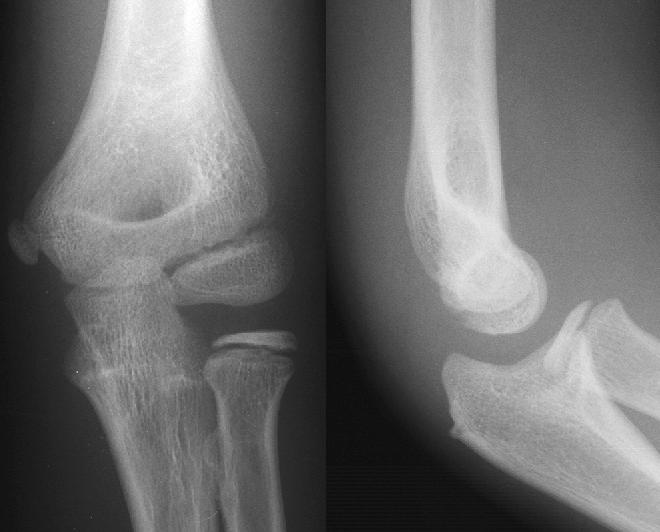
\includegraphics[height=0.25\linewidth]{images/x-ray.png}
   \caption[X-ray image]{An X-ray image of an elbow. Image taken from Wikipedia}
   \label{fig:xRay}
\end{figure}


\subsection{Computed tomography}

Now we will examine another important imaging technique: \textbf{computed tomography}. In this technique, a X-ray beam penetrates a slice of the patient, and a detector on the other side measures the intensity of the residual beam. This procedure is then repeated with different angles of the detector, obtaining projections from many different directions and a two-dimensional integral of attenuation. From these intensity profiles, it is possible to reconstruct a two-dimensional image, displaying a gray value that is proportional to the attenuation. The voxel value is given in \textit{Hounsfield units (HU)}.

\begin{table}[htbp]
\centering
\caption{Sample values for HU}
\label{tbl:Hounsfield}
\begin{tabular}{@{}ll@{}}
\toprule
\textbf{HU}        & \textbf{Material}   \\ \midrule
-1000              & Air         \\
0                  & Water       \\
\textgreater1000   & Metals      \\
Between 50 and 100 & Bone tissue \\
\bottomrule
\end{tabular}
\end{table}

Now we can focus on the results obtained by this process. The raw data that results from series of X-ray scans is called \textit{sinogram}, which is simply a display of all different projections for a given slice stacked together.

\begin{figure}[htb] %  figure placement: here, top, bottom
   \centering
   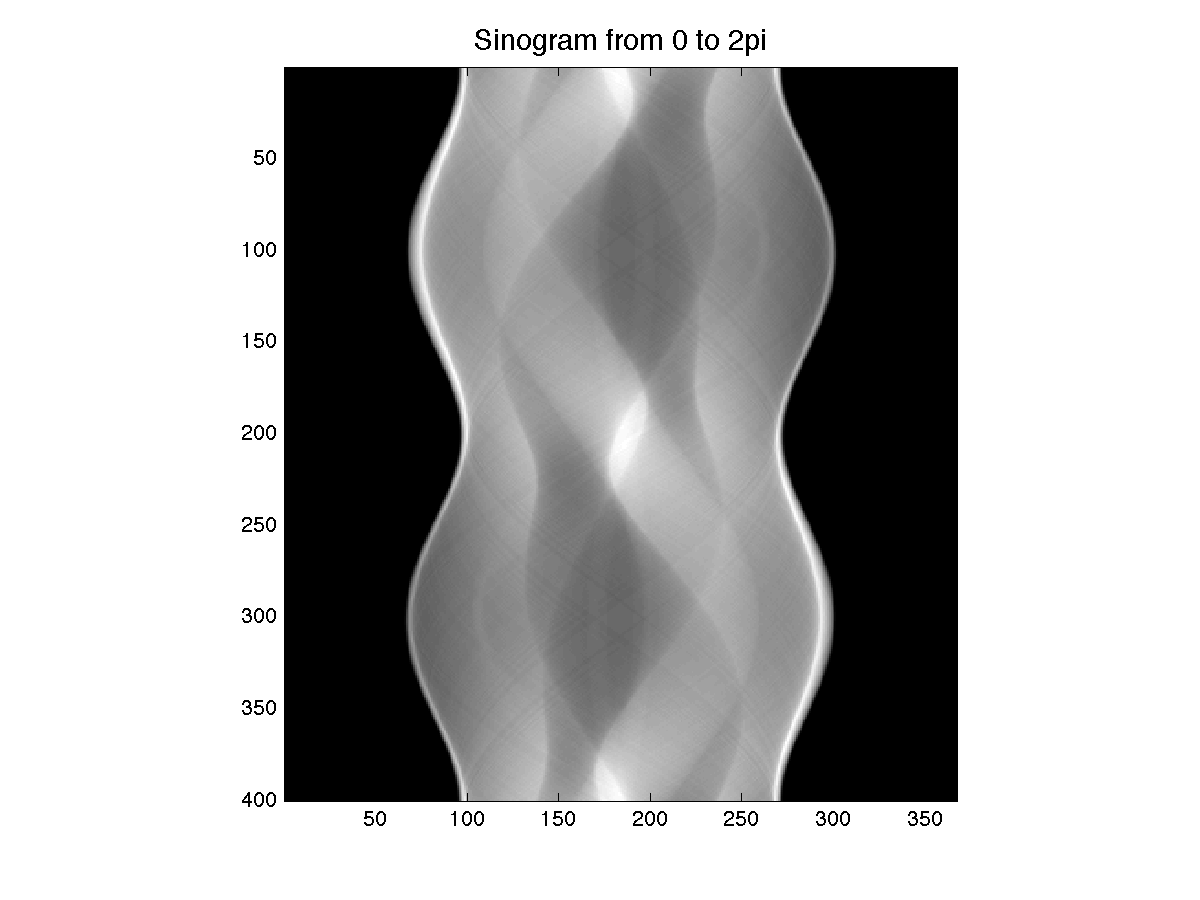
\includegraphics[width=0.45\linewidth]{images/sinogram.png}
   \caption[Sinogram]{A sinogram from a CT. It has sinusoidal undulations due to the CT tube rotations around the patient}
   \label{fig:sinogram}
\end{figure}

However, the sinogram is not sufficient for interpretation yet. So once the scan data has been acquired, it must be processed using a form of \textit{tomographic reconstruction}, which produces the series of images we were looking for.

\begin{figure}[htb] %  figure placement: here, top, bottom
   \centering
   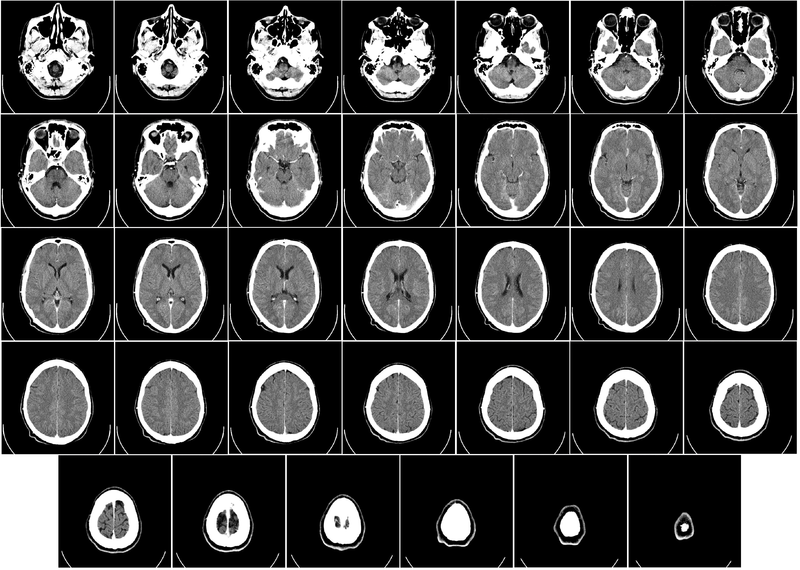
\includegraphics[width=0.45\linewidth]{images/Computed_tomography_of_human_brain.png}
   \caption[Computed tomography of human brain]{Computed tomography of human brain, from base of the skull to top. Image taken from Wikipedia}
   \label{fig:brainCT}
\end{figure}

Because CT scanners offer \textit{isotropic} (uniform in all orientations) or near isotropic, resolution, display of images does not need to be restricted to the conventional axial images. Instead, it is possible for a software program to build a volume by "stacking" the individual slices one on top of the other. We will discuss techniques for the volume rendering in Chapter~\ref{Chapter14} but it is important to remember that the idea of stacking the individual slices is at the basis of the work discussed in this thesis.

\subsection{Magnetic resonance tomography}

Now we will discuss images obtained using the \textbf{magnetic resonance tomography}. It works exploiting the magnetic moment of $^{1}$H nuclei bound in tissue water and fat molecules. With this technique, electromagnetic radiation in the radiofrequency range is transmitted to the body using a large magnet. The nuclei respond to the excitation by emission of RF signals with the same frequency, whose amplitude and phase are used for image construction. Information on slice location is obtained by superimposing spatial field gradients to the main magnetic field. As every voxel has a different frequency or phase we can divide signals coming from a single portion.\\

Imaging with this technique uses three independent processes:
\begin{itemize}
 \item \textbf{Selection of a slice}. With the application of a gradient on a given direction, we can observe that the frequency of the atoms linearly changes along that direction, so the body inside the magnet can be subdivided in parallel planes. When we apply the radiofrequency impulse it will excite only one plane leaving the other in the equilibrium state.
 \item \textbf{Frequency codification}. If we apply a gradient after the radiofrequency impulse and during the signal acquisition, the emission frequency of the protons varies linearly on the space. So the acquired signal is the sum of signals at different frequencies that can be obtained with a Fourier transform. When we associate a position with a single frequency we obtain the localization on a single dimension. However we need the phase codification for spin localization
 \item \textbf{Phase codification}. When we apply a gradient in the second spatial dimension after the radiofrequency impulse and before the acquisition, the spins along that direction will acquire a phase which can be easily measured. A single phase codification is not sufficient to obtain spatial information so the procedure should be repeated several times.
\end{itemize}

As a consequence of these processes, different impulse \textbf{sequences} lead to different images. The chosen sequence also determines the physical property that is represented into the resulting images. We will say that images representing different physical properties have different \textbf{contrast}

\begin{figure}[htb] %  figure placement: here, top, bottom
   \centering
   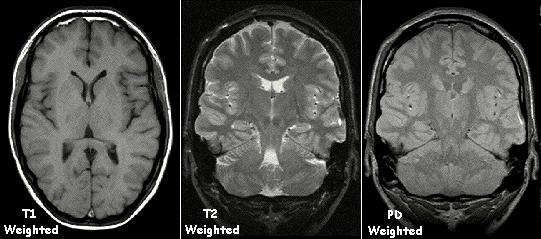
\includegraphics[width=0.50\linewidth]{images/mri.jpg}
   \caption[MRI of human brain]{MRI images of a brain with different contrasts. (a) $T_{1}$ weighted (b) $T_{2}$ weighted (c) $PD$ weighted. Image taken from Wikipedia}
   \label{fig:brainMRI}
\end{figure}

\subsection{Ultrasound}
Now we will see how to exploit sound for the creation of our medical images. First of all, we should remember that sound is a longitudinal pressure wave based on compression and decompression of the carrier medium. Therefore, the speed of sound $c$ depends on the compressibility and density of the carrier medium and its value is:
\begin{equation}
 c = \lambda \nu
\end{equation}
For tissues (excluding bones where the speed is higher) the average value is \textit{c = 1540 m/s}. While passing the body, the acoustic signal can be affected by \textit{reflection} on tissue boundaries, \textit{refraction} on border structures and \textit{scattering} (which occurs on structures with sizes comparable to the wavelength of sound and with different density). These effects cause misinterpretation in positions and extension of the studied structures. Also signal attenuation can have a role in this process.\\

Now we can see how to produce the acoustic signals for the images. They are generated using the \textit{inverse piezoelectric effect}. According to the \textit{direct piezoelectric effect} phenomenon, voltage can be measured in certain solids under deformation; on the other hand, we have the inverse effect when applying voltage to these solids we cause the deformations.\\
When we want to produce images, A piezoelectric US transducer transforms an electrical pulse into an acoustic signal which penetrates the object and is reflected on internal structures. The \textit{echoes} of the reflected pulses are detected by the transducer and converted back to electronic signals. This imaging technique is called \textbf{amplitude modulation} or \textbf{A-mode ultrasound imaging}. The percentage of reflected waves is dependent from the difference in acoustic impedance of the tissue involved. As this difference is usually small, the main part of the sound energy passes the boundary surfaces, making possible localization of organs lying behind each other by measuring the temporal distance between the echoes. The distance z of a boundary surface is:
\begin{equation}
 z = \frac{ct}{2}
\end{equation}
Where $t$ is the return time of the echo signal. However, echoes with longer run time are weaker due to absorption so they should be amplified.\\

As the A-mode technique only provides one-dimensional information, other imaging methods were developed. One of the most important is \textbf{B-mode} or \textbf{brightness modulation}. With this technique the echo amplitudes are converted to gray values in a two-dimensional image.\\

US imaging is also able to display flow speeds of fluids (such as blood) exploiting the \textit{Doppler effect}. This effect, consists in a shift of frequencies of a wave when its source is moving away from (or moving towards) an observer. A typical example is the shift in sound waves when an ambulance approaches with a siren. In US imaging, red blood cells can be seen as a source of ultrasound waves when they reflect the input signal. The frequency difference which results from the Doppler effect is:
\begin{equation}
 \Delta \nu = 2 \nu (\pm \frac{v}{c})
\end{equation}
Where $v$ is the velocity of blood. For Doppler ultrasound usually two techniques are used:
\begin{itemize}
 \item \textbf{Color Doppler}: we have informations regarding mean speed of the medium (good for a wide volume study)
 \item \textbf{Gated Doppler}: we obtain the spectrum of every speed in the medium (well suited for a detailed study)
\end{itemize}

\begin{figure}[htb] %  figure placement: here, top, bottom
   \centering
   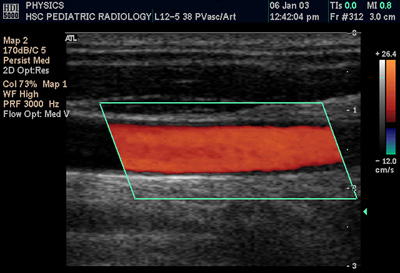
\includegraphics[width=0.40\linewidth]{images/ColourDopplerA.jpg}
   \caption[Color Doppler]{Color Doppler of a carotid artery. As we can see Ultrasound images usually have a low resolution (we typically have $256\times256$ with 8 bit per pixel). Image taken from Wikipedia}
   \label{fig:ultrasound}
\end{figure}

\subsection{Nuclear medicine and molecular imaging}

Now we will examine several medical imaging techniques which exploit \textit{nuclear medicine}. The main difference with x-ray diagnostics, is that the ionizing radiation is emitted by the patient rather than an outside instrument. For visualization of metabolic activities in organs we commonly use the \textit{tracer method}. With this method the radio nuclide (the \textit{tracer}) is bound to a chemical complex taken up by the organ like any metabolic substance, for example $^{99}$Tc is used in most applications. After it is injected, the tracer releases $\gamma-$radiations due to the decay of the nuclide which are detected and displayed as image intensities. Observing the distribution of this activity, we can visualize the metabolism of an organ. As a consequence, these methods show the physiological function of the system, not its structure. So we can merge images obtained with these techniques with images taken with other modalities to acquire more anatomical informations. The common term used for imaging the distribution of radioactivity is \textbf{scintigraphy}.\\

A particular scintigraphy based technique is \textbf{SPECT}, which uses rotating $\gamma-$cameras. Projections of the activity distribution are recorded at discrete angles and used for reconstruction of a three-dimensional volume. Another technique is \textbf{PET}, which uses positron ($\beta^{+}$) emitters as tracers. These kind of tracers are nuclides with an excess number of protons compared to the number of neutrons, so they are unstable and decay by converting a proton $p$ into a positron $e^{+}$, a neutron $n$ and a neutrino $\nu$, as stated by the following equation:
\begin{equation}
 p \rightarrow e^{+} + \nu + n
\end{equation}
This is known as the $\beta^{+}$ \textit{decay}. We cannot detect directly the positrons as their free path before annihilation is very small, however we can detect the $\gamma-$rays coming from the annihilation of the positron with an electron (which produces exactly two $\gamma-$quanta). To distinguish the annihilation $\gamma-$quanta from quanta resulting from other processes, we can use \textit{co-incidence detection}. So only events where two quanta are detected simultaneously are counted.\\

Image reconstruction with PET is similar to the one of CT even thought in this case the raw data set is of lower quality

\begin{figure}[htb] %  figure placement: here, top, bottom
   \centering
   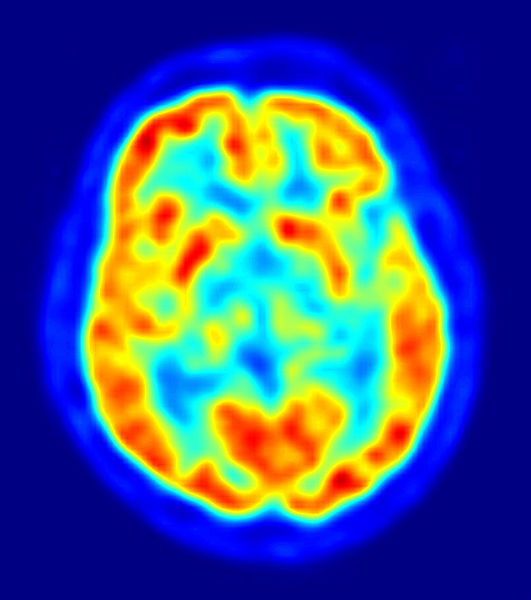
\includegraphics[width=0.30\linewidth]{images/PET.jpg}
   \caption[PET scan of a brain]{PET scan of a human brain. Image taken from Wikipedia}
   \label{fig:pet}
\end{figure}

\section{The need for three-dimensional representations}\label{sec13:3drepresentations}

At this point, we have collected a general overview of the medical imaging field. Therefore, we can examine typical uses in the everyday world. \cite{Stytz} offers a good case of study. In this example are collected 63 MRI image slices of the head from a patient with intractable seizure activity. From these slices the doctor cannot disclose an abnormality. After the reconstruction of a three-dimensional model of the MRI, a study reveals flattening in the gyri of the lower motor and sensory strips. So the doctor asks for a second study using a PET to portray the metabolic activity of the brain. Using these images it is also possible to build a three-dimensional model of the average cortical metabolic activity. According to it, the patients has hypermetabolic activity; however as the PET has a poor resolution, the location of the abnormality cannot be correlated with surface anatomical landmarks. So the doctor has to combine the 3D MRI model with the 3D PET model, using post-hoc image registration techniques to align the two sets of data. With these representations, the doctor can also use a surgery test program to simulate surgery on the brain model and after the operation the patient's seizure activity cease.\\

Another interesting use of three-dimensional models consists in the \textbf{printing of human parts with a 3D printer}.
The following case study comes from \cite{Zopf}. In February of 2012, a medical team at the University of Michigan carried out an unusual operation on a three month old boy. In fact he was born with a rare condition called \textit{tracheobronchomalacia}, which causes weakness in the tissue of the airway. This made breathing very difficult causing also blockage of vital blood vessels. The area of weak tissue would have somehow needed to be repaired or replaced with a dangerous operation for a patient so young. As a consequence, they decided to print a \textit{tracheal splint} with a 3D printer. The researchers began by taking a CT scan of the baby's chest which they converted into a three-dimensional model. Using this model they designed and printed the splint with biocompatible materials. After the implantation, problems with the tracheobronchomalacia disappeared.
As we can see, without a technique for the three-dimensional representation of models, the researchers would have not been able to build the splint.

\begin{figure}[htb] %  figure placement: here, top, bottom
   \centering
   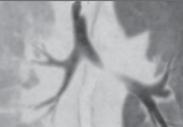
\includegraphics[width=0.33\linewidth]{images/TrachealSplint0.png}\hfill
   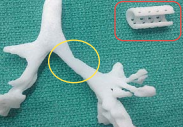
\includegraphics[width=0.33\linewidth]{images/TrachealSplint1.png}\hfill
   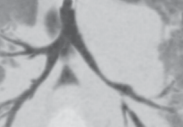
\includegraphics[width=0.33\linewidth]{images/TrachealSplint2.png}
   \caption[3D print of a tracheal splint]{3D print of a tracheal splint. (a) The 3D printed models for the airway and for the splint. (b) The airway in expiration before placement of the splint. (c) The airway in expiration one year after placement of the splint. Images taken from~\cite{Zopf}}
   \label{fig:TrachealSplint}
\end{figure}

As we can read in \cite{Himi}, three-dimensional models can also be used for postoperative investigations. For example in that work the authors created a model from helical CT scans of the temporal bone for investigations in cochlear implantation.\\

However these are only a few examples of things we can do with three-dimensional representations of human parts. Later we will study a good technique to produce perfect models
